\section{Estado del Arte.}

\noindent
La comunicación es una necesidad básica en los seres humanos, no podemos coexistir sin poder manifestarnos con los demás. A través del tiempo hemos evolucionado nuestras maneras comunicativas por medio de artefactos que nos permiten facilitar el contacto con nuestros círculos sociales. Con la evolución tecnológica se permitió la creación de los Smartphones o teléfonos inteligentes, que nos permiten una cohesión social ya que está ligada a la red, -una de las principales causas de la globalización-, teniendo muchas funciones que permiten una comunicación más dinámica con diferentes colectivos, aunque estén en diferentes partes del mundo.

\noindent
\newline
Entre el año 2000 a 2004 el mercado de los Smartphone se expandió alrededor del mundo con sistemas de HTD, BlackBerry o RIM, pero no fue hasta 2007, cuando Apple aparece con su línea de celulares IPhone, que el mercado de los smartphones evolucionó la industria de la telefonía móvil y de las comunicaciones en general, gracias principalmente a su experiencia en Internet, misma que posteriormente traería consigo la app store, una tienda virtual que permitía (y lo sigue haciendo) descargar aplicaciones para el celular, mismas que resolverían pequeñas tareas para el usuario, solucionando así aspectos de su vida cotidiana, pero no favoreciendo a tu cartera, pues en la mayoría de los casos, éstas tenían un costo monetario. 

\noindent
Sin embargo, como en todo mercado, surge competencia y se presenta Android de la compañía Google en mismo año del lanzamiento del IPhone, aunque Android en ese momento no causo tanto impacto hoy en día es el mayor competidor de Apple, ya que se volvió rotundamente exitoso, porque, a diferencia de la compañía de la manzana, se contaba con aplicaciones en su mayoría gratuitas. Además, el recién presentado sistema operativo gozaba de un gran punto a su favor: la compatibilidad con más de un fabricante de smartphones. 
Por otro lado, el resto de los sistemas competidores, como BlackBerrry o Symbian de Nokia perdieron fuerza y popularidad, dejando camino libre a Google y Apple.

\noindent
\newline
Con esta revolución se nos permite, por un lado, estar en contacto unos con otros en cualquier momento, en cualquier lugar, con cualquier persona; y, por el otro lograr tareas cotidianas de una manera más sencilla, en menor tiempo o con menor esfuerzo. \cite{Conexion}

\noindent
Ahora bien, si lo nos concentramos en los pros y contras de los dos titanes de los sistemas operativos móviles, debemos decir que es Android que, para bien o para mal, se lleva la corona, y no necesariamente por ser mejor, sino por ser más accesible, esto se demuestra de más de una forma, la primera: gente que posee un teléfono android antes que un iPhone, pues el sistema del androide verde en 2017 ha logrado casi un 81.7 por ciento del mercado global, seguido muy distantemente de su competidor principal, que casi alcanzó un 12 por ciento en el segundo trimestre del mismo año.		
El segundo aspecto es su alta compatibilidad para con los desarrolladores de aplicaciones, pues de trata de un sistema operativo sistemas de código abierto, no cerrado. El usuario no tiene que conocer esta característica, pero es importante de cara al 
mercado, ya que un software de código abierto es gratis y accesible a todo el mundo. Esto es especialmente útil, como ya se mencionaba, para los desarrolladores, quienes pueden experimentar y probar, mientras que cada fabricante puede introducir sus particularidades. \cite{IDC}

\noindent
\newline
Dicho todo la anterior, quedan claro dos aspectos fundamentales para el desarrollo del presente proyecto: que la comunicación por medio de celulares es de suma importancia en la actualidad y, que un potencial mercado para la misma es aquel en donde la empresa de la gran G promueve sus servicios.

\noindent
Así, ponemos los pies sobre la tierra y nos situamos en nuestro presente, regresamos a la problemática mencionada capítulos anteriores y analizamos las aplicaciones que presentan propuestas y soluciones similares en el mercado, pero éstas ya disponibles en el mercado.
De éstas, la mayoría se desarrollan para en el ámbito de la educación superior y se centran en que el alumno de las respectivas instituciones esté informado sobre las situaciones escolares.
A continuación, enlistamos dichas aplicaciones, mencionando además sus características más relevantes.

\pagebreak
\subsection{NET ANAHUAC}

	\begin{figure}[htbp!]
		\centering
		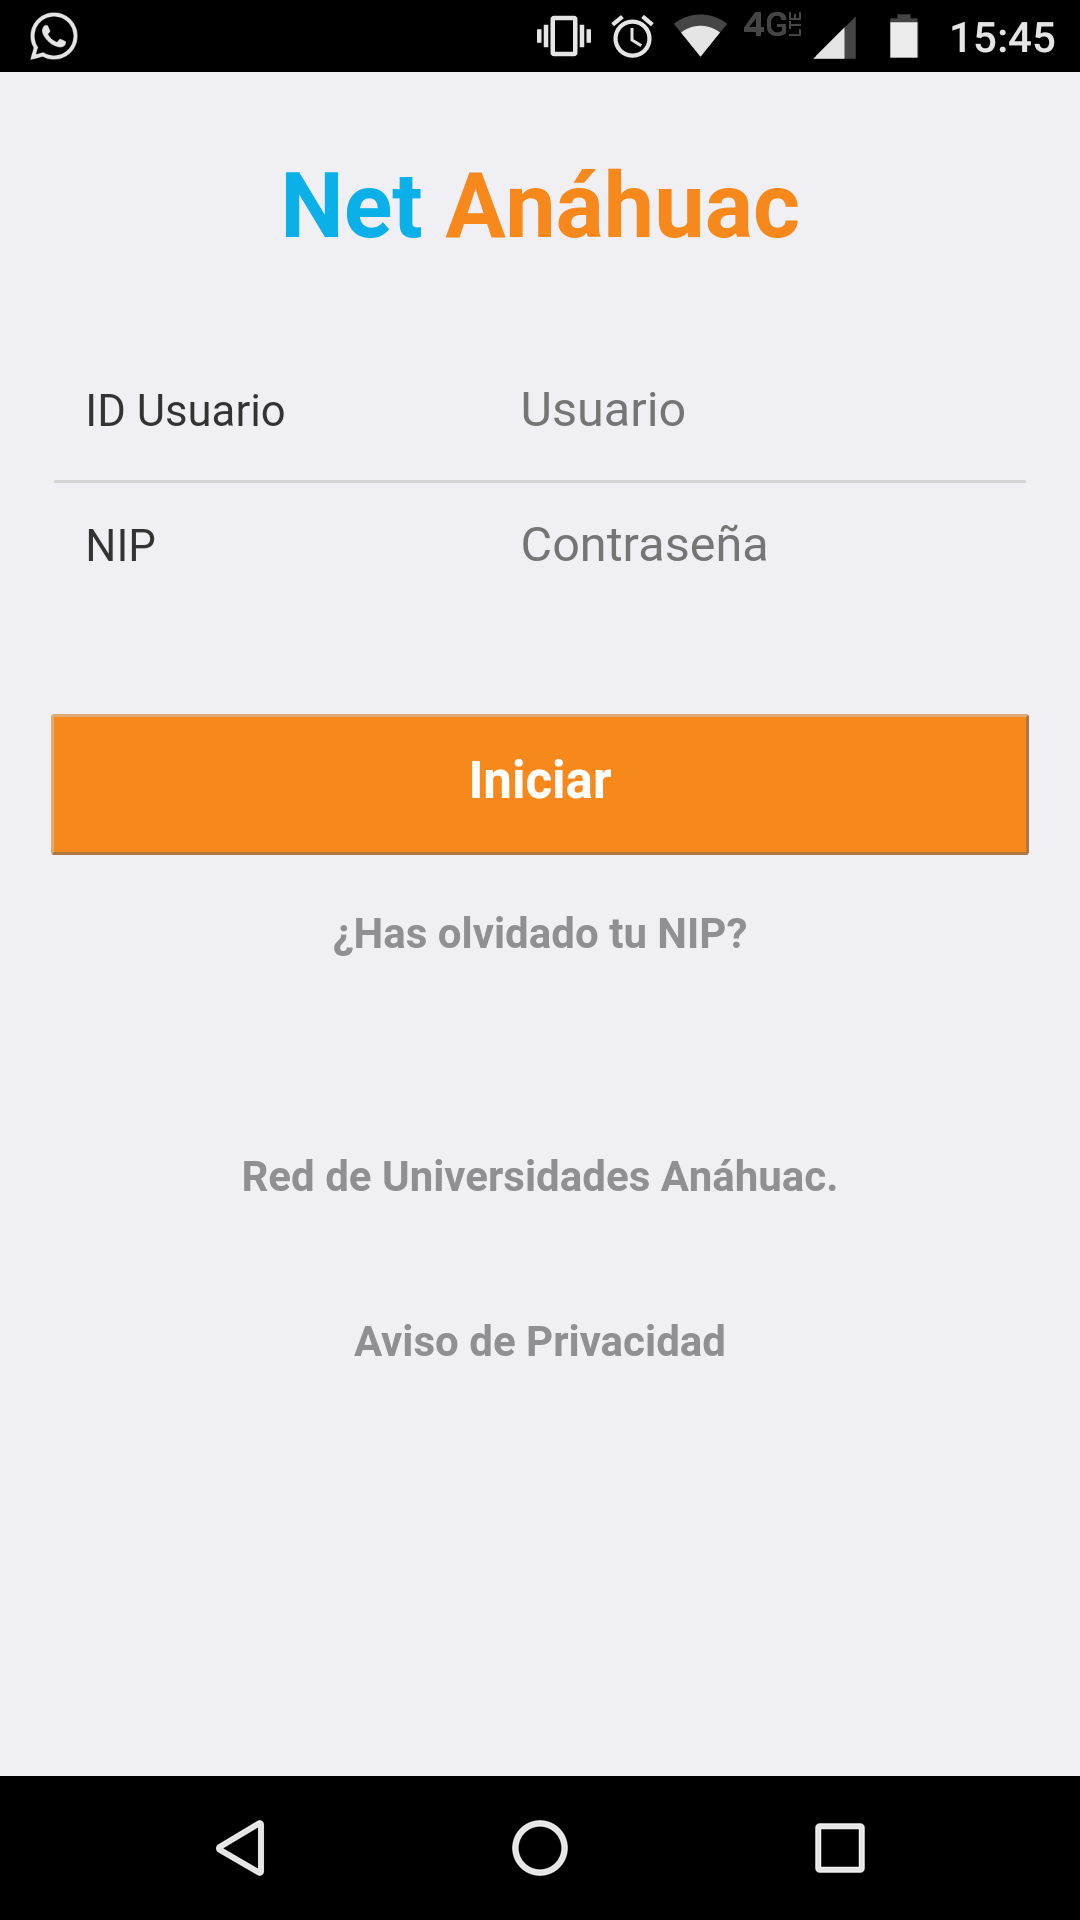
\includegraphics[width=0.3\textwidth]{estado_arte/fotosarte/4}
		\caption{Página Inicial NetAnahuac.}
		%\caption{Diseño inconcluso de la base de datos.}
	\end{figure}

	\noindent
	Esta aplicación, que se encuentra disponible para IOS y Android, está hecha para la Universidad Anáhuac y conecta a todos los usuarios de las escuelas de la Anahuac en toda la república, se puede consultar en cualquier momento y en cualquier lugar.
	El estudiante puede obtener información precisa y actualizada sobre los acontecimientos de su escuela, sólo necesita un usuario y una contraseña de la Intranet Anáhuac, el mismo que se utiliza comúnmente en el sistema institucional.
	Ofreciod por: Fomento e Investigación Integral S.C..
	Completa suite de Servicios Académicos y Financieros para la red de Universidades Anáhuac en México.

	\begin{table}[!htb]
		\centering
		\caption{NET ANAHUAC}
		\label{red_anahuac}
		\begin{tabular}{@{}|c|c|c|@{}}
		\toprule
		Características Académicas & Información Financiera & Otros  
		\\ \midrule
			\begin{tabular}[c]{@{}c@{}}
				-Búsqueda de Cursos,\\ -Cursos Planeados,\\ -Cita de Inscripción,\\ -Horario,\\ -Perfil,\\ -Situación Académica,\\ -Calificaciones Parciales,\\ -Historia Académica,\\ -Mi Avance.
			\end{tabular} & 
			\begin{tabular}[c]{@{}c@{}}
				-Estado de Cuenta,\\ -Crédito Educativo,\\ -Apoyo Financiero,\\ -Retenciones.
			\end{tabular} & 
			\begin{tabular}[c]{@{}c@{}}
				-Noticias,\\ -Eventos
			\end{tabular}\\ \bottomrule
		\end{tabular}
	\end{table}

\pagebreak
\subsection{MIT MOBILE}

	\begin{figure}[htbp!]
		\centering
		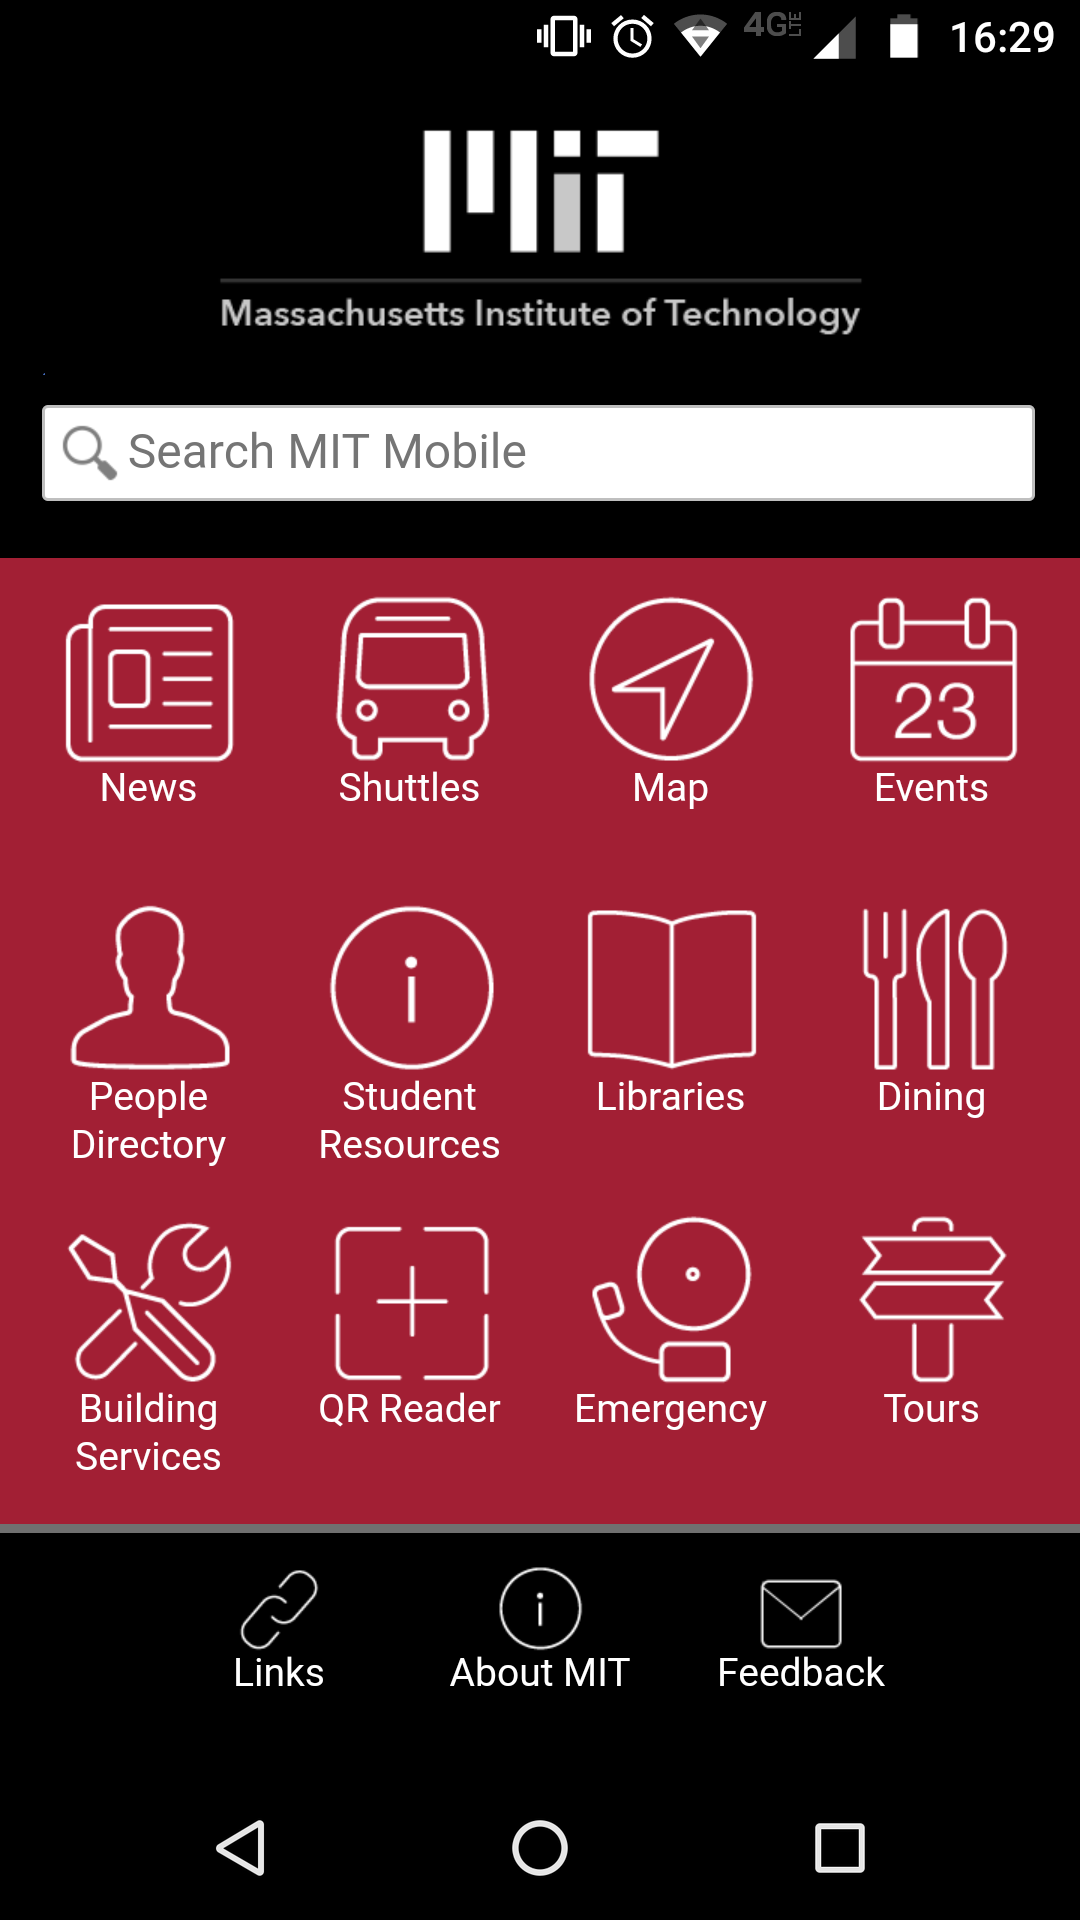
\includegraphics[width=0.3\textwidth]{estado_arte/fotosarte/5}
		\caption{Página Inicial MIT MOBILE.}
	\end{figure}

	\noindent
	El ''MIT Mobile Experience Lab'', aplicación destinada al Massachusetts Institute of Technology (MIT), utiliza dispositivos móviles personales para desbloquear el potencial en el mundo físico que rodea a los integrantes de la comunidad universitario de Massachusetts. Busca, en sus palabras, reinventar radicalmente y diseñar creativamente las conexiones entre personas, así como la información y los lugares a los que éstos acceden y visitan frecuentemente. \cite{MIT}
		
 	\begin{table}[htbp!]
		\centering
		\caption{MIT MOBILE}
		\label{mit_mobile}
		\begin{tabular}{|c|}
			\hline
			Características \\ \hline
			\begin{tabular}[c]{@{}c@{}}
				-Noticias del Campus,\\ -Búsqueda del mapa del campus,\\ -Calendario de Eventos,\\ -Búsqueda de Directorio,\\ -Información sobre el MIT\\ -Información sobre campus de emergencias\\ -Menú de comidas\\ -Reportes\\ -Scanner QR.
			\end{tabular} \\ \hline
		\end{tabular}
	\end{table}
	
\pagebreak
\subsection{CONEXIÓN UVM}	

	\begin{figure}[htbp!]
		\centering
		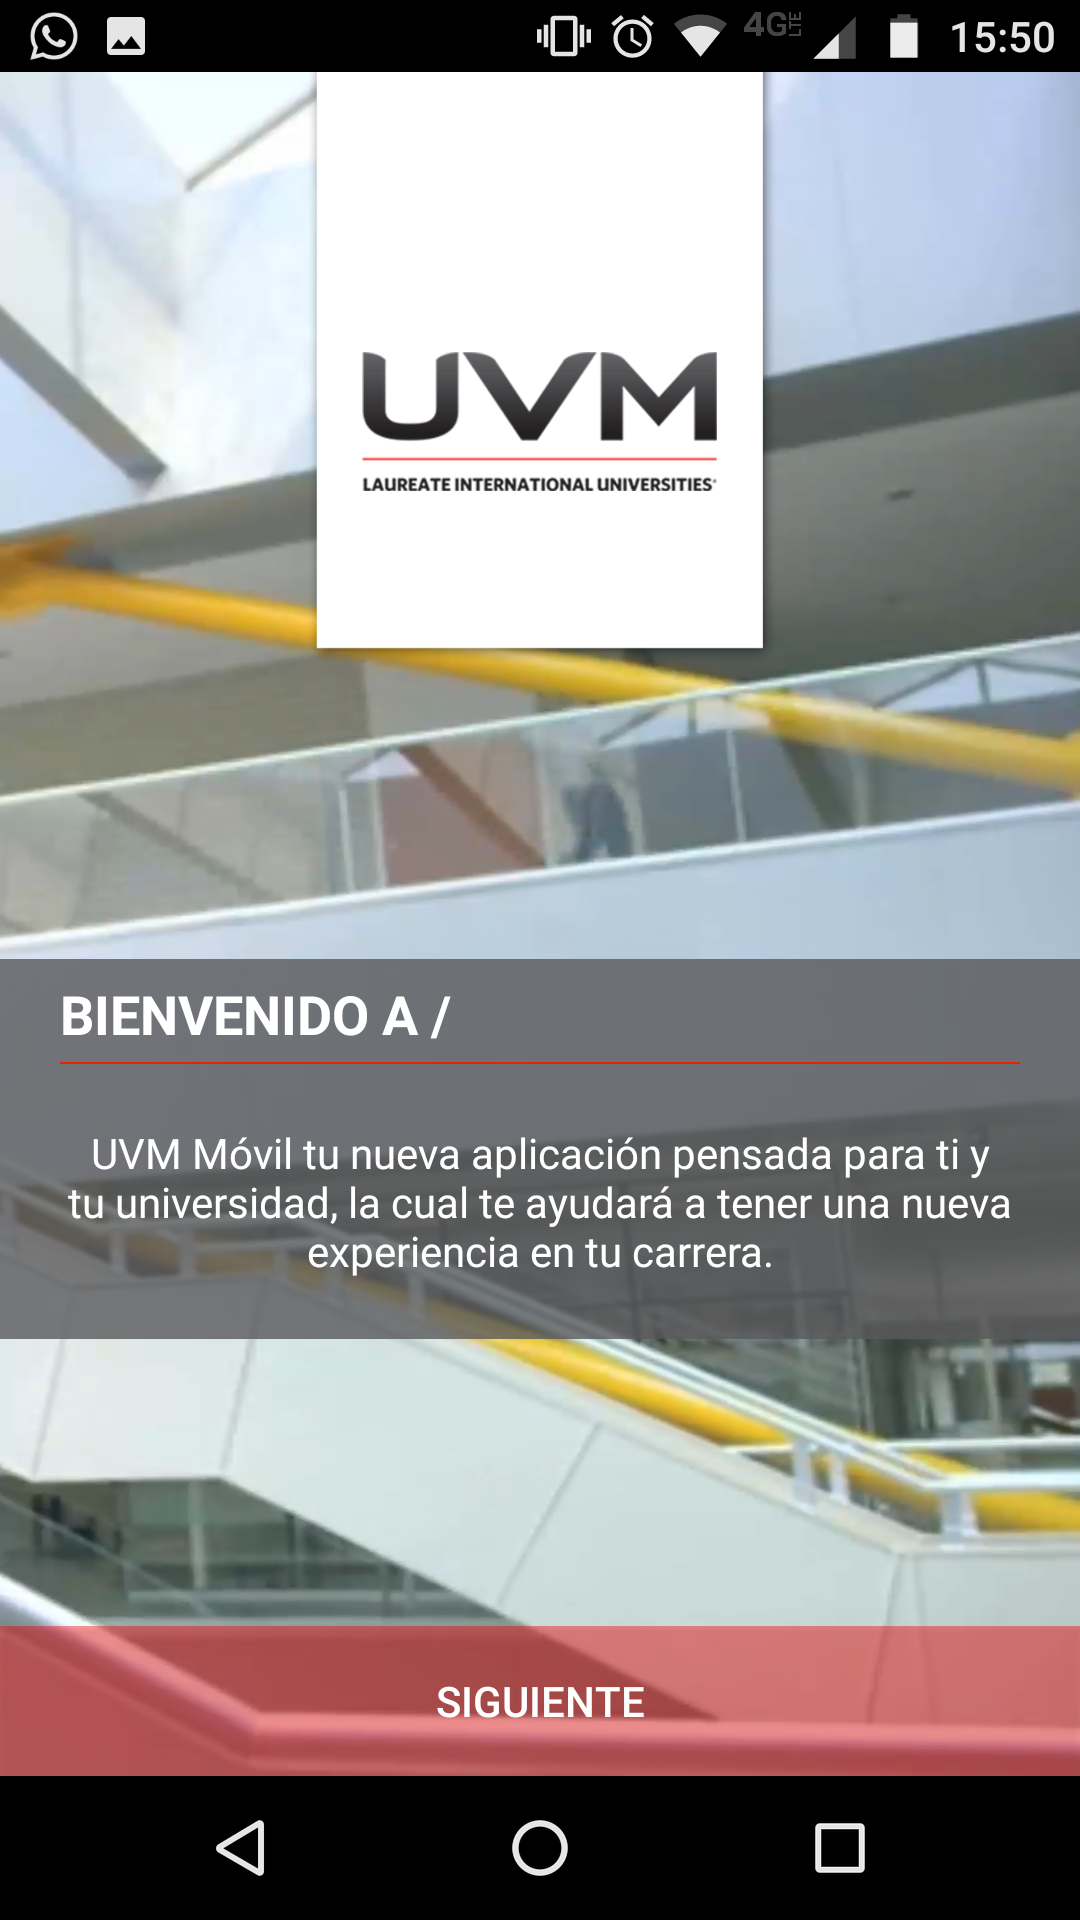
\includegraphics[width=0.3\textwidth]{estado_arte/fotosarte/6}
		\caption{Página Inicial de Conexión UVM.}
	\end{figure}

	\noindent
	Solución móvil de la UVM que soporta el proceso de toma y consulta de asistencia, así como la consulta de calificaciones en línea de los alumnos en curso; además de proveer un medio de comunicación directa entre la comunidad estudiantil, docente y administrativa a través del envío de notificaciones, encuestas y mensajes. \cite{conexion_uvm} Disponible para iOS y Android.

 	\begin{table}[htbp!]
		\centering
		\caption{CONEXIÓN UVM}
		\label{conexion_uvm}
		\begin{tabular}{|c|}
		\hline
		Características \\ \hline
			\begin{tabular}[c]{@{}c@{}}
				-Consulta de Asistencia,\\ -Consulta de Calificaciones,\\ -Medio de comunicación entre la comunidad estudiantil,\\  -Notificaciones,\\ -Comunicación entre estudiantes y profesores.
			\end{tabular} \\ \hline
		\end{tabular}
	\end{table}

\pagebreak
\subsection{IBERO MOVIL}

	\begin{figure}[htbp!]
		\centering
		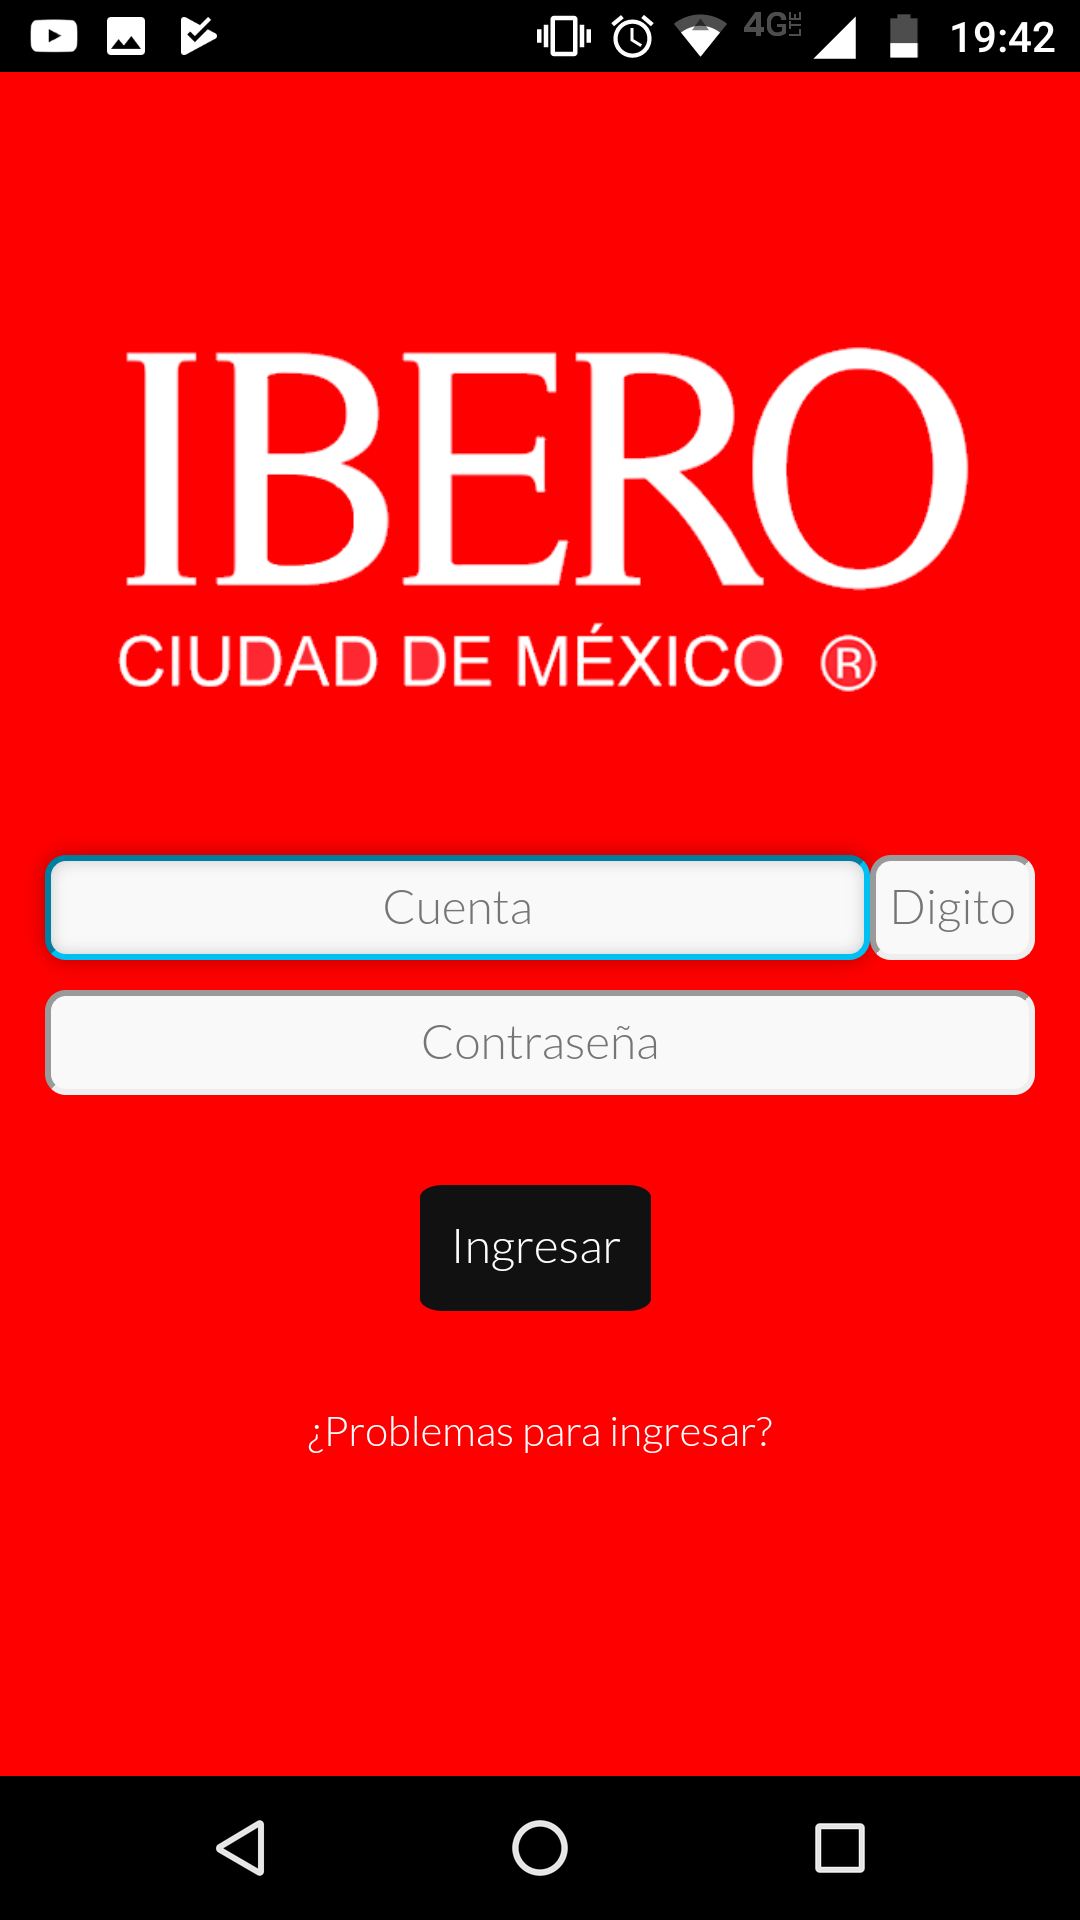
\includegraphics[width=0.3\textwidth]{estado_arte/fotosarte/ibero}
		\caption{Página Inicial de Ibero Móvil.}
	\end{figure}
			
	\noindent
	Ibero Móvil es la aplicación de la Universidad Iberoamericana, en la Ciudad de México, para acceder a la información académica de los estudiantes de la institución y a los estados de cuenta, así como realizar la reinscripción de las materias para los alumnos en cada nuevo curso. En esta app podrás: Consultar tu Historia Académica, Consultar tus Materias Inscritas, Consultar tu Situación Académica, -Consultar tu Estado de Cuenta, Consultar el Calendario de la Ibero, Consultar tu Adeudos, Consultar tus Estados de Cuenta por Servicio, Reinscribir tus materias para el siguiente semestre, Realizar Pagos de tus Adeudos, Actualizar tu Información en Biblioteca. Fue realizada por la Dirección de Informática y Telecomunicaciones. Se encuentra disponible para Android, iOS y Windows Phone.	\cite{ibero}
		
	\begin{table}[htbp!]
		\centering
		\caption{IBERO MOVIL}
		\label{ibero_movil}
		\begin{tabular}{|c|}
			\hline
			Características \\ \hline
			\begin{tabular}[c]{@{}c@{}}
				-Búsqueda de Cursos,\\ -Cursos Planeados,\\ -Cita de Inscripción,\\ -Horario,\\ -Perfil,\\ -Situación Académica,\\ -Calificaciones Parciales,\\ -Historia Académica,\\ -Mi Avance
			\end{tabular} \\ \hline
		\end{tabular}
	\end{table}

\pagebreak	
\subsection{MANIFEST ESCOM}

	\begin{figure}[htbp!]
		\centering
		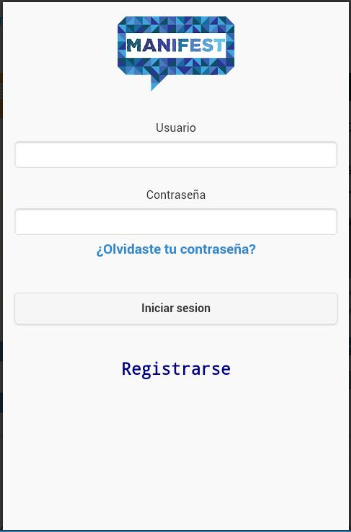
\includegraphics[width=0.3\textwidth]{estado_arte/fotosarte/ManifestESCOM}
		\caption{Página Inicial de Manifest ESCOM.}
	\end{figure}

	\noindent
	Manifest, es una aplicación diseñada para mantenerte al tanto de los últimos acontecimientos que ocurren en la Escuela Superior de Cómputo (ESCOM) y así seguir los temas de interés para la comunidad. Te tiene actualizado sobre los diferentes tipos de publicaciones: eventos, cursos, convocatorias, noticias, avisos urgentes, entre otros...
	Además, puedes personalizar la aplicación para recibir las publicaciones, dependiendo el perfil que tengas (alumno ESCOM, alumno Posgrado, profesor, personal de apoyo y egresado). Disponible para Android mediante la descarga del APK. \cite{manifest}
	
	\begin{table}[htbp!]
		\centering
		\caption{MANIFEST ESCOM}
		\label{my-label5}
		\begin{tabular}{|c|}
			\hline
			Características \\ \hline
			\begin{tabular}[c]{@{}c@{}}
				-Eventos,\\ -Cursos,\\ -Convocatorias,\\ -Noticias,\\ -Avisos Urgentes.
			\end{tabular} \\ \hline
		\end{tabular}
	\end{table}

\noindent
\newline
\newline
Así, una vez mencionadas las aplicaciones similares a la nuestra, es momento de presentar, de igual forma, la propuesta que tenemos, sus características y posibilidades. Se trata de ESCOMobile, y se describe aquí debajo.

\pagebreak
\subsection{ESCOMobile}

	\begin{figure}[htbp!]
		\centering
		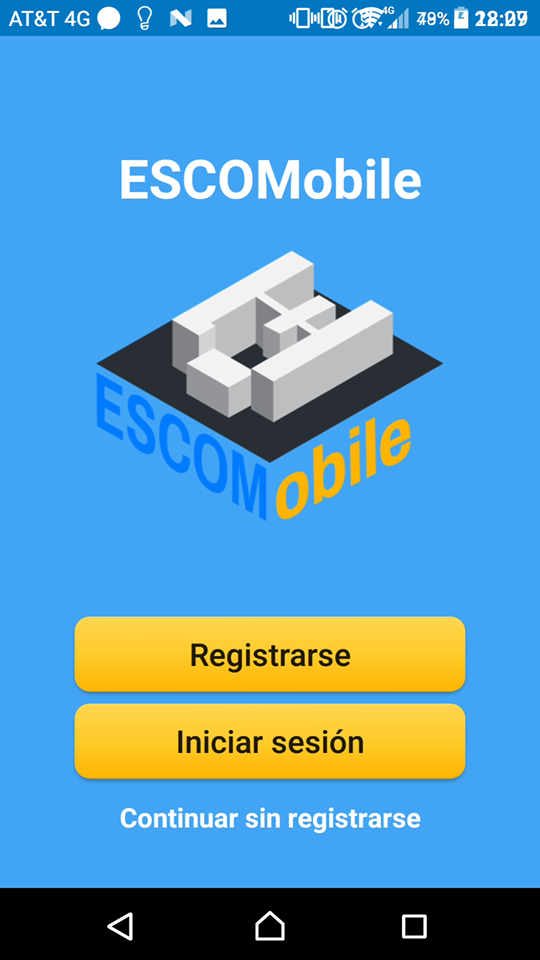
\includegraphics[width=0.3\textwidth]{estado_arte/fotosarte/ESCOMobile}
		\caption{Página Inicial de ESCOMobile.}
	\end{figure}

	\noindent
	ESCOMobile es una aplicación móvil para dispositivos Android, destinada a la comunidad de ESCOM (alumnos y profesores), que permitirá una mayor interacción de los alumnos de la institución con su entorno, esto engloba diversos aspectos, como conocer la distribución de los salones y áreas académicas de la escuela, consultar la información de los profesores del plantel, generar citas para tratar aspectos escolares, o bien, mantenerse al día sobre las ofertas de trabajo disponibles para los estudiantes a través de la bolsa de trabajo de ESCOM. La aplicación se encuentra disponible para alumnos, profesores e invitados (quienes no se encuentras inscritos en la ESCOM, por ejemplo, padres de familia). 
	
 	\begin{table}[htbp!]
		\centering
		\caption{ESCOMobile}
		\label{ESCOMobile}
		\begin{tabular}{|c|}
			\hline
			Características \\ \hline
			\begin{tabular}[c]{@{}c@{}}
				-Registro Alumnos y Profesores,\\ -Consulta del mapa de la ESCOM,\\ -Consulta de áreas académicas a través del mapa,\\ -Consulta de los profesores de ESCOM por medio de perfiles,\\ Consulta de horarios y estadísticas de profesores,\\ -Citas con profesores,\\ Consulta de la bolsa de trabajo disponible para ESCOM,\\ -Acceso a Invitados.
			\end{tabular} \\ \hline
		\end{tabular}
	\end{table}

\noindent
\newline
Finalmente, ya que conocemos las características que ESCOMobile y las aplicaciones similares presentan, mostramos una comparativa de las mismas, enlistando en una tabla que las aplicaciones descritas y las principales características que éstas tienen. Como se observa a continuación. 

\begin{tablaCCCCCCC}
		{Características}{Red Anahuac}{MIT Mobile}{Ibero Móvil}{Conexión UVM}{Manifest ESCOM}{ESCOMobile}{IDTabla4}
		\CCCCCCCitem{Registro de usuarios}			{x}{x}{x}{x}{x}{x}
		\CCCCCCCitem{Mapa del Campus}				{ }{x}{ }{ }{ }{x}
		\CCCCCCCitem{Ubicar áreas en el mapa}		{ }{ }{ }{ }{ }{x}
		\CCCCCCCitem{Búsqueda de Cursos}			{x}{x}{x}{x}{x}{ }
		\CCCCCCCitem{Consulta de profesores}		{ }{ }{ }{ }{ }{x}
		\CCCCCCCitem{Información de profesores}		{ }{ }{ }{ }{ }{x}
		\CCCCCCCitem{Opinar sobre profesores}		{ }{ }{ }{ }{ }{x}
		\CCCCCCCitem{Cita de Inscripción}			{x}{ }{x}{x}{ }{ }
		\CCCCCCCitem{Calificaciones Parciales}		{x}{x}{x}{x}{x}{ }
		\CCCCCCCitem{Estado de Cuenta}				{x}{ }{x}{x}{ }{ }
		\CCCCCCCitem{Eventos}						{x}{x}{x}{ }{ }{ }
		\CCCCCCCitem{Generación de Citas}			{ }{ }{ }{ }{ }{x}
		\CCCCCCCitem{Consulta a ofertas de trabajo}	{ }{ }{ }{ }{ }{x}
		\CCCCCCCitem{Mensajería Alumno - Profesor}	{ }{ }{ }{x}{ }{ }
		\CCCCCCCitem{Acceso a invitados}			{ }{x}{ }{ }{ }{x}	
\end{tablaCCCCCCC}

\noindent
Así, es claro que todas las aplicaciones son muy similares entre sí, pero cada una brinda un enfoque diferente para un público determinado. Teniendo claro el público al cual va dirigido ESCOMobile y los objetivos de la misma app, es posible decir que las características que proporciona son las idóneas, que se trabaja en ellas y en que lleguen de forma adecuada al usuario final, teniendo siempre presente su razón de ser y tomando además la iniciativa de evolucionar siempre para mejorar. 